\documentclass{article}
\usepackage{graphicx} % Required for inserting images
\usepackage[top=0.9in, bottom=1in, left=1.5in, right=1.5in]{geometry}
\usepackage[utf8]{inputenc}
\usepackage[icelandic]{babel}
\usepackage[T1]{fontenc}
\usepackage[sc]{mathpazo}
\usepackage[parfill]{parskip}
\renewcommand{\baselinestretch}{1.2}
% Tables and lists
\usepackage{booktabs,tabularx}
\usepackage{multirow}
\usepackage{enumerate}
\usepackage{adjustbox}
\usepackage{multicol}
\usepackage{xcolor}
\usepackage{algpseudocode}
\usepackage{algorithm}
\usepackage{tikz}
\usepackage{nicefrac}
\usepackage{changepage}
\usepackage{fancyvrb}
\usepackage{xlop}
\usepackage{titlesec}
\usetikzlibrary{arrows, positioning, calc, graphs}

% Math
\usepackage{amsmath, amsfonts, amssymb, amsthm}
% Graphics

\usepackage{graphicx}
\usepackage{tikz}
% Code environment
\usepackage{minted}
%\usepackage{bm}
%\usepackage{siunitx}
%\usepackage{animate}
%\usepackage{hyperref}
%\usepackage{movie15}
%\usepackage{multicol}
%\usepackage{changepage}
\title{Formal Languages and Computability 6}
\author{Ragnar Björn Ingvarsson, rbi3}
\tikzset{->, >=stealth', shorten >=1pt, node distance=2cm,thick, main node/.style={circle,draw,minimum size=3em}}


\begin{document}
\renewcommand\thepage{}
	
	\maketitle

	\newpage
	\setcounter{page}{1}
	\renewcommand\thepage{\arabic{page}}

	\section{Let $\Sigma=\{0,1\}$ and consider $A = \{01^n01^n\mid n\geq0\}$. 
	First show if $A$ is regular or not. If $A$ is nonregular languages, 
	give a CFG or a PDA to show that it is context free.}
	To prove that the language is nonregular we use pumping lemma.

	Let $s = 01^p01^p$, and we get three cases for the splitting into $xyz$:

	\begin{itemize}
		\item{$y=0$:} Here, for $xy^iz$ we can say that $i=2$ and we get the 
			string $001^p0^p$ which is not in $A$ so here lies a contradiction.
		\item{$y=01^k$, $k < p$:} Here we can pump to any $i>1$ and get 
			$(01^k)^i1^{p-k}01^p$ which is clearly not in $A$ so we get a 
			contradiction.
		\item{$y=1^k$, $k < p$:} Here we can pump until the number of y's 
			exceeds $p$ by saying $i=p+1$, and we get a contradiction since 
			such a string is not in $A$.
	\end{itemize}

	We see that for the string $s=01^p01^p$ all three cases lead to a 
	contradiction, bringing us to the conclusion that $A$ is nonregular.

	We can then give a CFG to show that it is context free and such a CFG 
	would look like this:
	\[S\rightarrow 0A\]
	\[A\rightarrow 1A1\mid 0\]
	Where $S$ is the starting state.

	\section{Let $A$ denote the language that corresponds to checking 
	whether the Hamming distance between two binary strings is three. 
	Show that $A$ is CFL by constructing a PDA that recognizes it.}

	\begin{center}
	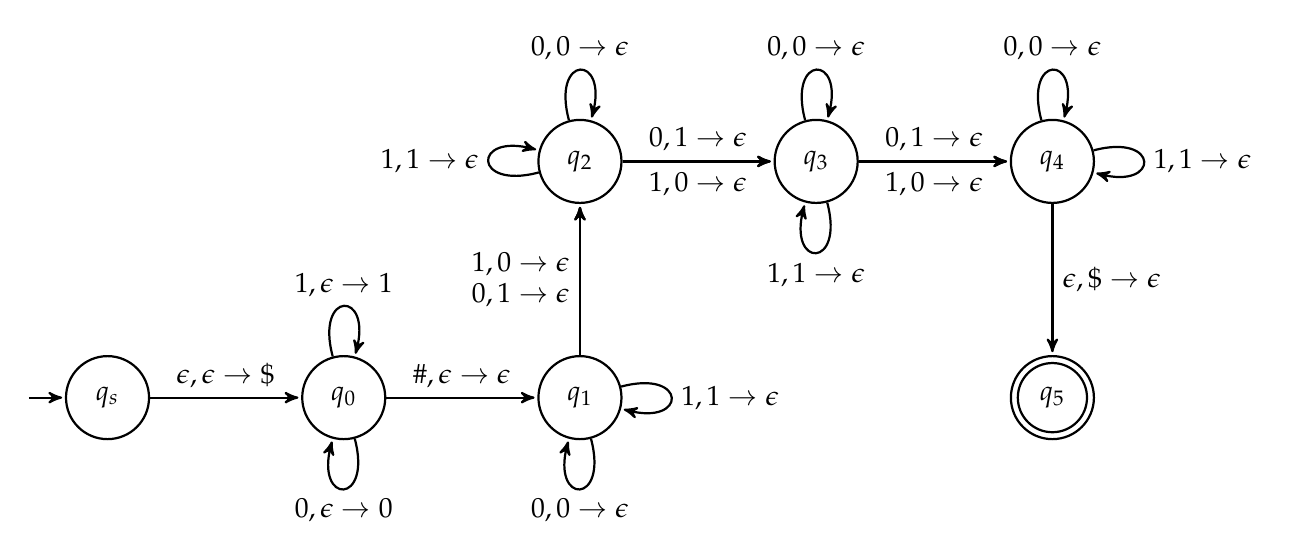
\begin{tikzpicture}[thick]
		\node[main node] at (-3,0) (qs) {$q_s$};
		\node[main node] at (0,0) (q0) {$q_0$};
		\node[main node] at (3,0) (q1) {$q_1$};
		\node[main node] at (3,3) (q2) {$q_2$};
		\node[main node] at (6,3) (q3) {$q_3$};
		\node[main node] at (9,3) (q4) {$q_4$};
		\node[main node] at (9,0) (q5) {$q_5$};
		\node[main node, minimum size=2.5em] at (9,0) (q5fin) {};

		\path (-4,0) edge node {} (qs);
		\path (qs) edge[above] node {$\epsilon,\epsilon\rightarrow\$$} (q0);
		\path (q0) edge[loop above=20] node {$1,\epsilon\rightarrow 1$} (q0);
		\path (q0) edge[loop below=20] node {$0,\epsilon\rightarrow 0$} (q0);
		\path (q0) edge[above] node {$\#,\epsilon\rightarrow\epsilon$} (q1);
		\path (q1) edge[loop right=20] node {$1,1\rightarrow\epsilon$} (q1);
		\path (q1) edge[loop below=20] node {$0,0\rightarrow\epsilon$} (q1);
		\path (q1) edge[left,pos=0.4] node {$0,1\rightarrow\epsilon$} (q2);
		\path (q1) edge[left,pos=0.6] node {$1,0\rightarrow\epsilon$} (q2);
		\path (q2) edge[loop left=20] node {$1,1\rightarrow\epsilon$} (q2);
		\path (q2) edge[loop above=20] node {$0,0\rightarrow\epsilon$} (q2);
		\path (q2) edge[above] node {$0,1\rightarrow\epsilon$} (q3);
		\path (q2) edge[below] node {$1,0\rightarrow\epsilon$} (q3);
		\path (q3) edge[loop below=20] node {$1,1\rightarrow\epsilon$} (q3);
		\path (q3) edge[loop above=20] node {$0,0\rightarrow\epsilon$} (q3);
		\path (q3) edge[above] node {$0,1\rightarrow\epsilon$} (q4);
		\path (q3) edge[below] node {$1,0\rightarrow\epsilon$} (q4);
		\path (q4) edge[loop right=20] node {$1,1\rightarrow\epsilon$} (q4);
		\path (q4) edge[loop above=20] node {$0,0\rightarrow\epsilon$} (q4);
		\path (q4) edge[right] node {$\epsilon,\$\rightarrow\epsilon$} (q5);
	\end{tikzpicture}
	\end{center}

	\section{Suppose that a CS student wants to encode events taking place 
	in an ice-hockey game to a string using alphabet $\Gamma =  \{a,b,c,1,2,3,x, y,\mid\}$.}

	\begin{itemize}
		\item[a)] Let $A$ denote the language corresponding to all valid 
			strings. Show that $A$ is a regular language. 

			First we will give a RE for one period.
			\[
				((1\mid 2\mid 3)(a\mid b\mid c))\mid((a\mid b\mid c)(1\mid 2\mid 3))(x^*y^*(a\mid b\mid c)^*(1\mid 2\mid 3)^*)^*
			\]
			We can then denote this regular expression as $p$ and then just 
			say that the regular expression for the whole game is 
			\[p\hspace{0.5em}"\hspace{-0.3em}\mid\hspace{-0.2em}"\hspace{0.2em}p_1 \hspace{0.5em}"\hspace{-0.3em}\mid\hspace{-0.2em}"\hspace{0.2em}p_2\]
		\item[b)] Let $B$ denote those interesting games where at no point 
			in time either team leads by more than 1 goal. Is $B$ regular 
			or nonregular?

			This is regular as we can give a rough outline of a NFA that 
			describes it:

			\begin{center}
				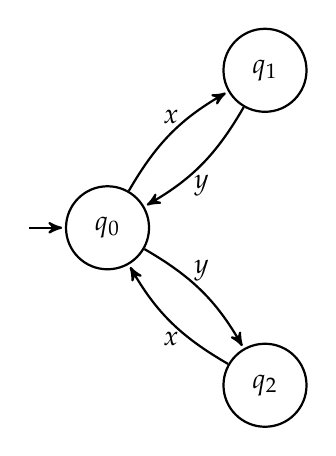
\begin{tikzpicture}[thick]
					\node[main node] (q0) {$q_0$};
					\node[main node] at (2,2) (q1) {$q_1$};
					\node[main node] at (2,-2) (q2) {$q_2$};

					\path (-1,0) edge node {} (q0);
					\path (q0) edge[bend left=15] node[above] {$x$} (q1);
					\path (q1) edge[bend left=15] node[below] {$y$} (q0);
					\path (q0) edge[bend left=15] node[above] {$y$} (q2);
					\path (q2) edge[bend left=15] node[below] {$x$} (q0);
				\end{tikzpicture}
			\end{center}

			Here, the $q_0$ state is for the score being 0-0, the $q_1$ for 
			1-0 and $q_2$ for 0-1, where each state is a NFA that describes 
			a normal game and each transition is to and from the same state 
			within those NFA's. With this we can ensure that at no point in 
			time does the lead ever get greater than 1 and we can see 
			that this can be described with a NFA so it is regular.
		\item[c)] Plus-minus statistic is an often used performance metric: 
			a goal means +1 for the wing, and when the opponent scores the 
			wing on ice receives -1. Let $C$ denote the games where home 
			team's 1st wing has a positive plus-minus statistic. Show that 
			$C$ is context-free.

			We show that it is context-free by giving a PDA for it, and to 
			begin with we can give a NFA for a single period with two states 
			for determining if $a$ is on the ice or not. I choose here 
			to make a NFA since it never interacts with the stack as we 
			need the stack to count the plus-minus statistic.
	\begin{center}
		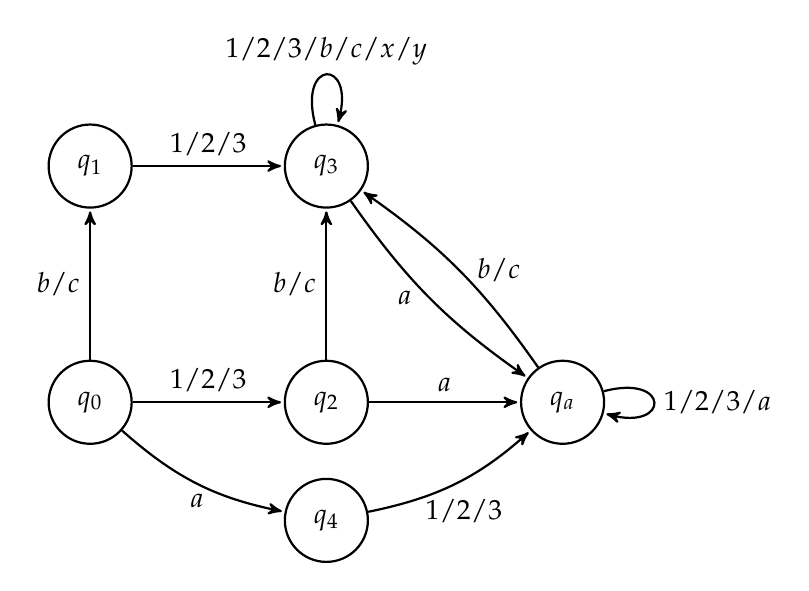
\begin{tikzpicture}[thick]
			\node[main node] at (0,0) (q0) {$q_0$};
			\node[main node] at (0,3) (q1) {$q_1$};
			\node[main node] at (3,0) (q2) {$q_2$};
			\node[main node] at (3,3) (q3) {$q_3$};
			\node[main node] at (3,-1.5) (q4) {$q_4$};
			\node[main node] at (6,0) (qa) {$q_a$};

			\path (q0) edge[left] node {$b/c$} (q1);
			\path (q0) edge node[above] {$1/2/3$} (q2);
			\path (q1) edge node[above] {$1/2/3$} (q3);
			\path (q2) edge node[left] {$b/c$} (q3);
			\path (q0) edge[bend right=15] node[below] {$a$} (q4);
			\path (q4) edge[bend right=15] node[below=.2em,xshift=0.3em] {$1/2/3$} (qa);
			\path (q2) edge node[above] {$a$} (qa);
			\path (q3) edge[bend right=10] node[left=.3em] {$a$} (qa);
			\path (qa) edge[bend right=10] node[right=.3em] {$b/c$} (q3);
			\path (q3) edge[loop above=20] node {$1/2/3/b/c/x/y$} (q3);
			\path (qa) edge[loop right=20] node {$1/2/3/a$} (qa);
		\end{tikzpicture}
	\end{center}

	Notice that we dont define any start or end states since this is only 
	going to be part of the whole PDA. We will then name this chunk $P$ 
	for period and we can then link up a whole game with such a NFA:

	\begin{center}
		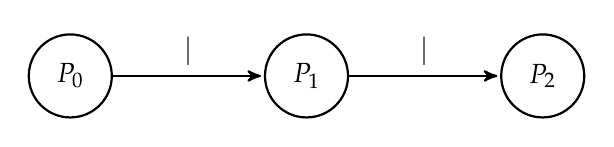
\begin{tikzpicture}[thick]
			\node[main node] at (0,0) (p0) {$P_0$};
			\node[main node] at (3,0) (p1) {$P_1$};
			\node[main node] at (6,0) (p2) {$P_2$};

			\path (p0) edge node[above] {$\mid$} (p1);
			\path (p1) edge node[above] {$\mid$} (p2);
		\end{tikzpicture}
	\end{center}

	Where each $P$ state has a transition from both $q_3$ and $q_a$ to the 
	$q_0$ state of the next $P$ on the symbol "$\mid$".

	Now, we can have two instances of this NFA called $X$ and $Y$. Then 
	we can draw out the final PDA consisting of these two states along with 
	a start state $q_s$ and finish state $q_f$.

	\begin{center}
		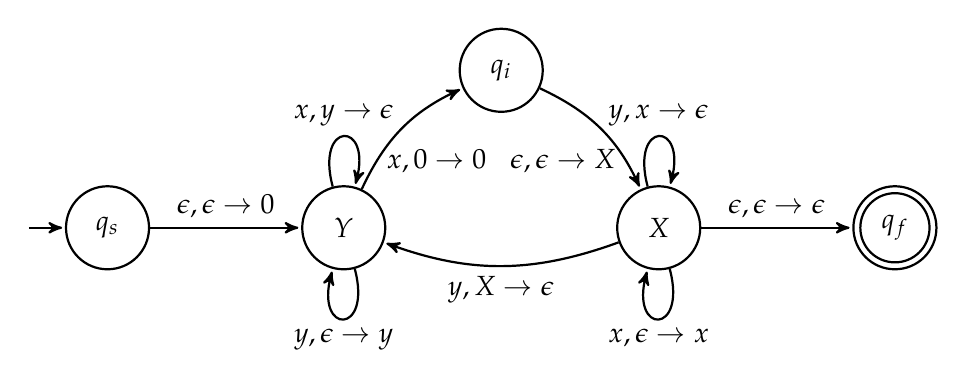
\begin{tikzpicture}[thick]
			\node[main node] at (0,0) (qs) {$q_s$};
			\node[main node] at (3,0) (qy) {$Y$};
			\node[main node] at (5,2) (qi) {$q_i$};
			\node[main node] at (7,0) (qx) {$X$};
			\node[main node] at (10,0) (qf) {$q_f$};
			\node[main node,minimum size=2.5em] at (10,0) (qffin) {};

			\path (-1,0) edge node {} (qs);
			\path (qs) edge node[above] {$\epsilon,\epsilon\rightarrow0$} (qy);
			\path (qy) edge[loop above=20] node[above] {$x,y\rightarrow\epsilon$} (qy);
			\path (qy) edge[loop below=20] node[below] {$y,\epsilon\rightarrow y$} (qy);
			\path (qy) edge[bend left=20] node[right,pos=.2] {$x,0\rightarrow0$} (qi);
			\path (qi) edge[bend left=20] node[left,pos=.8] {$\epsilon,\epsilon\rightarrow X$} (qx);
			\path (qx) edge[bend left=20]  node[below] {$y,X\rightarrow\epsilon$} (qy);
			\path (qx) edge[loop above=20] node[above] {$y,x\rightarrow\epsilon$} (qx);
			\path (qx) edge[loop below=20] node[below] {$x,\epsilon\rightarrow x$} (qx);
			\path (qx) edge node[above] {$\epsilon,\epsilon\rightarrow\epsilon$} (qf);
		\end{tikzpicture}
	\end{center}

	Where aside from the paths leading from and to the start and end state, 
	all paths only travel from $q_a$ to $q_a$, in the corresponding period. 
	Then there is the path from the start state which leads to the $q_0$ 
	state in the first period of $q_y$ and the end state where to we can 
	travel from the $q_3$ or $q_a$ state in the final period of $q_x$.

	The paths relating to the intermittent state $q_i$ are as such; the 
	path to $q_i$ is from $q_a$ and the path from $q_i$ is to $q_a$ of 
	$X$ in the same period as was in $Y$.

	The logic here is that we have two states of the game, negative and 
	positive, $Y$ and $X$. When we are situated in $Y$, the negative 
	state, we can be sure that our stack contains no plus scores, that is, 
	$x$'s. And the reverse is also true that when we are in $X$, no $y$'s 
	are in the stack. This ensures that we know the exact state of the game 
	at any given time instead of having to count the score at the end.
	\end{itemize}

	\end{document}
